\documentclass[10pt,a4paper]{article}

\usepackage[utf8]{inputenc}
\usepackage[T5]{fontenc}
\usepackage{amsmath, amssymb, amsfonts}
\usepackage[a4paper, top=12mm, bottom=12mm, left=15mm, right=15mm]{geometry}
\usepackage{graphicx}
\usepackage{xcolor}
\usepackage{booktabs, tabularx, array}
\usepackage{colortbl}
\usepackage{float}
\usepackage{fancyhdr}
\usepackage{enumitem}
\usepackage[unicode, colorlinks=true, linkcolor=primary, citecolor=secondary, urlcolor=secondary]{hyperref}

\emergencystretch=3em
\tolerance=2000
\hbadness=10000
\hfuzz=2pt
\setlength{\parskip}{2pt}
\setlength{\parindent}{0pt}

\definecolor{primary}{RGB}{0, 45, 98}
\definecolor{secondary}{RGB}{0, 102, 153}
\definecolor{tablehead}{RGB}{228, 238, 250}

\makeatletter
\renewcommand{\section}{\@startsection{section}{1}{\z@}%
  {-1.5ex \@plus -0.4ex \@minus -.2ex}%
  {0.6ex \@plus .1ex}%
  {\normalfont\normalsize\bfseries\color{primary}}}
\renewcommand{\subsection}{\@startsection{subsection}{2}{\z@}%
  {-1.1ex\@plus -0.3ex \@minus -.1ex}%
  {0.4ex \@plus .1ex}%
  {\normalfont\small\bfseries\color{secondary}}}
\makeatother

\setlength{\headheight}{13pt}
\pagestyle{fancy}
\fancyhf{}
\fancyhead[L]{\footnotesize\textit{ĐHQGHN - Trường Đại học Công nghệ (UET)}}
\fancyhead[R]{\footnotesize\textit{Báo cáo Kỹ thuật: Phân vùng Bản đồ Nhà kho \& Điều hướng Giọng nói qua Microphone}}
\fancyfoot[C]{\footnotesize Trang \thepage/2}
\renewcommand{\headrulewidth}{0.4pt}

\renewcommand{\figurename}{Hình}
\renewcommand{\tablename}{Bảng}
\newcolumntype{Y}{>{\centering\arraybackslash}X}
\newcolumntype{R}{>{\raggedright\arraybackslash}X}

\begin{document}

% ==============================================================================
% TIÊU ĐỀ BÁO CÁO NGẮN GỌN (COMPACT HEADER CHO BÁO CÁO 2 TRANG)
% ==============================================================================
\begin{center}
  {\large\bfseries\color{primary} BÁO CÁO KỸ THUẬT: PHÂN VÙNG BẢN ĐỒ NHÀ KHO (WAREHOUSE SEGMENTATION)}\\[2pt]
  {\large\bfseries\color{primary} VÀ ĐIỀU HƯỚNG BẰNG GIỌNG NÓI TRỰC TIẾP QUA MICROPHONE VỚI NAV2}\\[3pt]
  {\footnotesize \textbf{Họ và tên:} Nguyễn Quang Tuân \quad|\quad \textbf{MSSV:} 23020767 \quad|\quad \textbf{GVHD:} PGS.TS. Hoàng Văn Xiêm, CN. Nguyễn Quốc Bảo}\\
  {\footnotesize \textbf{Nền tảng:} ROS 2 Humble, Gazebo Fortress, OpenCV, Nav2, Faster-Whisper \& Live Microphone STT \quad|\quad \textbf{GitHub:} \url{https://github.com/Tuan404cl/Turtlebot_sim_test4}}
\end{center}
\vspace{-5pt}
\noindent\textcolor{primary}{\rule{\linewidth}{0.8pt}}

% ==============================================================================
% MỤC 1: PHÂN VÙNG BẢN ĐỒ NHÀ KHO & GẮN NHÃN NGỮ NGHĨA
% ==============================================================================
\section{Phương Pháp Phân Vùng Bản Đồ Nhà Kho (Map Segmentation) \& Gắn Nhãn Ngữ Nghĩa}

\subsection{Quy trình xử lý ảnh Occupancy Grid 2D của Nhà kho bằng OpenCV}
Bản đồ lưới chiếm dụng 2D của nhà kho (\texttt{maps/map.pgm} và \texttt{maps/map.yaml}) có kích thước $W \times H = 603 \times 1003\text{ pixels}$, độ phân giải $r = 0.05\text{ m/pixel}$ và gốc tọa độ $(x_0, y_0) = (-15.1, -25.1)\text{ m}$. Module \texttt{map\_segmentation.py} thực hiện chuỗi 4 bước xử lý ảnh tự động để phân chia toàn bộ không gian bên trong nhà kho ($x \in [-10.0, 12.5]\text{ m}, y \in [-22.1, 16.8]\text{ m}$) thành 05 khu vực vận hành kho vận:
\begin{enumerate}[leftmargin=14pt, itemsep=1pt, topsep=1pt]
  \item \textbf{Phân ngưỡng nhị phân (Binary Thresholding):} Tách vùng không gian trống di chuyển được ($I(u,v) \ge 250 \rightarrow 255$) khỏi tường bao/vách kệ ($I(u,v) = 0$) và vùng lõi kệ hàng kín ($I(u,v) = 205$).
  \item \textbf{Lọc hình thái học (Morphological Filtering):} Áp dụng phép mở (\texttt{MORPH\_OPEN}, kernel Ellipse $3\times 3$) và phép đóng (\texttt{MORPH\_CLOSE}, kernel Rect $5\times 5$) nhằm khử nhiễu điểm quét LiDAR và làm liền mạch đường biên của dãy kệ ngang phía Bắc và 3 dãy kệ dọc phía Nam.
  \item \textbf{Biến đổi khoảng cách Euclid (Distance Transform):} Tính trường khoảng cách $D(u,v) = \text{dist}(u,v) \times r$ từ mỗi điểm trống đến tường hoặc kệ hàng gần nhất bằng \texttt{cv2.distanceTransform(DIST\_L2)}, đảm bảo tọa độ đích của từng khu vực luôn nằm tại vùng thông thoáng cách xa vật cản ($D(u,v) \ge 1.70\text{ m}$).
  \item \textbf{Phân vùng Watershed có điều khiển hạt giống (Marker-Controlled Watershed):} Khởi tạo các vùng hạt giống tại 05 phân khu chức năng của nhà kho và áp dụng \texttt{cv2.watershed} trên phổ gradient đảo của trường khoảng cách để xác định ranh giới tự nhiên tại các lối giao.
\end{enumerate}

\vspace{-5pt}
\begin{figure}[H]
  \centering
  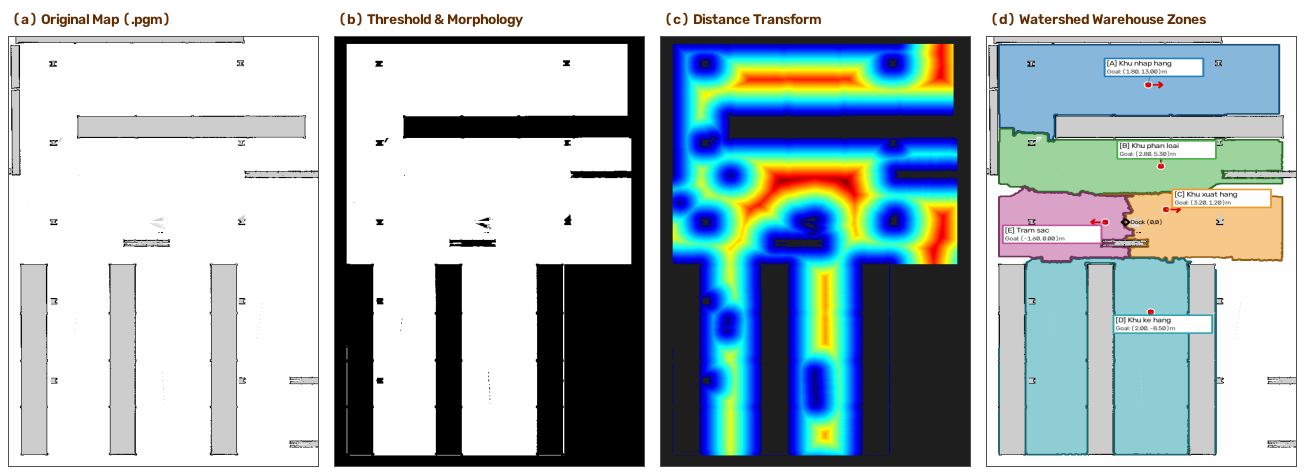
\includegraphics[width=0.73\textwidth]{figures/map_segmentation_pipeline.png}
  \vspace{-8pt}
  \caption{\footnotesize Quy trình 4 bước xử lý ảnh phân vùng bản đồ Nhà kho (\texttt{map.pgm}) và gắn nhãn 05 khu vực vận hành \texttt{A, B, C, D, E}.}
  \label{fig:pipeline}
\end{figure}
\vspace{-8pt}

\subsection{Quy đổi tọa độ Pixel sang ROS Map và lưu trữ dữ liệu khu vực nhà kho}
Với gốc ảnh $(u=0, v=0)$ ở góc trên bên trái và gốc bản đồ ROS $(x_0, y_0)$ ở góc dưới bên trái, công thức chuyển đổi song ánh giữa tọa độ pixel $(u, v)$ và tọa độ thực $(x, y)$ trong hệ quy chiếu \texttt{map} là:
\begin{equation}
  x = x_0 + (u + 0.5) \times r, \qquad y = y_0 + (H - 1 - v + 0.5) \times r
\end{equation}
Toàn bộ thông tin 05 khu vực được xuất ra \texttt{config/semantic\_regions.json} và \texttt{config/semantic\_regions.yaml}, đồng thời hiển thị trực tiếp dưới dạng nhãn 3D \texttt{MarkerArray} (\texttt{/semantic\_regions\_markers}) trên giao diện RViz2.

\vspace{-3pt}
\begin{table}[H]
  \centering
  \scriptsize
  \caption{\footnotesize Bảng thông số 05 khu vực chức năng nhà kho trong \texttt{semantic\_regions.json} và \texttt{semantic\_regions.yaml}.}
  \vspace{-3pt}
  \renewcommand{\arraystretch}{1.10}
  \begin{tabularx}{\textwidth}{c l R c c c c}
    \toprule
    \rowcolor{tablehead}
    \textbf{ID} & \textbf{Tên khu vực nhà kho} & \textbf{Từ khóa giọng nói nhận diện (Aliases)} & \textbf{Pixel $(u, v)$} & \textbf{Tọa độ ROS $(x, y, \text{yaw})$} & \textbf{Diện tích} & \textbf{Clearance} \\
    \midrule
    \textbf{A} & Khu nhập hàng & \texttt{khu vực a, khu nhập hàng, kho nhập hàng} & $(338, 240)$ & $(1.80, 13.00, 0.00)$ & $155.07\text{ m}^2$ & $3.00\text{ m}$ \\
    \textbf{B} & Khu phân loại & \texttt{khu vực b, khu phân loại, kiểm hàng} & $(358, 394)$ & $(2.80, 5.30, 1.57)$ & $105.86\text{ m}^2$ & $2.70\text{ m}$ \\
    \textbf{C} & Khu xuất hàng & \texttt{khu vực c, khu xuất hàng, khu đóng gói} & $(366, 476)$ & $(3.20, 1.20, 0.00)$ & $71.82\text{ m}^2$ & $1.93\text{ m}$ \\
    \textbf{D} & Khu kệ hàng & \texttt{khu vực d, khu kệ hàng, kho lưu trữ} & $(342, 670)$ & $(2.00, -8.50, -1.57)$ & $203.32\text{ m}^2$ & $2.90\text{ m}$ \\
    \textbf{E} & Trạm sạc & \texttt{khu vực e, trạm sạc, khu điều phối} & $(270, 500)$ & $(-1.60, 0.00, 3.14)$ & $60.98\text{ m}^2$ & $1.70\text{ m}$ \\
    \bottomrule
  \end{tabularx}
\end{table}
\vspace{-4pt}

% ==============================================================================
% MỤC 2: NHẬN DẠNG GIỌNG NÓI TRỰC TIẾP QUA MICROPHONE & ĐIỀU HƯỚNG VỚI NAV2
% ==============================================================================
\section{Nhận Dạng Giọng Nói Trực Tiếp Từ Microphone \& Điều Hướng Đa Chặng Với Nav2}

\subsection{Thu âm trực tiếp từ Microphone \& Nhận dạng tiếng Việt (\texttt{voice\_command\_node.py})}
Thay vì sử dụng các file âm thanh tạo sẵn, node \texttt{voice\_command\_node} thu nhận tín hiệu giọng nói \textbf{trực tiếp từ Microphone phần cứng} trên máy tính ở định dạng chuẩn PCM 16kHz, 16-bit Mono qua giao tiếp ALSA/PulseAudio (\texttt{arecord}). Khi khởi động, hệ thống tự động kích hoạt và chuẩn hóa mức âm lượng thu (90\%) cho Digital Microphone tích hợp (\texttt{sof-hda-dsp DMIC}). Hệ thống hỗ trợ hai chế độ thu trực tiếp: (1) \textbf{Push-to-Talk} (nhấn phím \texttt{SPACE} hoặc \texttt{R} để thu câu lệnh 4 giây) và (2) \textbf{Auto-Listen VAD} (nhấn phím \texttt{M} để tự động lắng nghe liên tục khi năng lượng hiệu dụng $\text{RMS} \ge 0.012$). Luồng âm thanh thu từ Microphone được chuyển thành văn bản tiếng Việt qua \textbf{SpeechRecognition (\texttt{vi-VN})} kết hợp mô hình AI Offline \textbf{Faster-Whisper (\texttt{base-int8})} và publish lên topic \texttt{/voice\_command}.

\subsection{Giải thuật phân tích câu lệnh nhà kho \& điều hướng đa điểm (\texttt{voice\_navigation\_node.py})}
Node \texttt{voice\_navigation\_node} chuẩn hóa văn bản tiếng Việt và xử lý 3 lớp kịch bản điều hướng kho vận:
\begin{itemize}[leftmargin=14pt, itemsep=1pt, topsep=1pt]
  \item \textbf{Điều hướng đơn đích (\texttt{SINGLE\_GOAL}):} Với các câu lệnh như \textit{``Đi đến khu vực A''} hoặc \textit{``Đi đến khu nhập hàng''}, bộ phân tích ánh xạ tên khu vực sang tọa độ đích $(x, y, \text{yaw})$ trong \texttt{semantic\_regions.json} và gửi yêu cầu tới Nav2.
  \item \textbf{Điều hướng nhiều điểm đến (\texttt{MULTI\_WAYPOINT}):} Xử lý các câu lệnh phức hợp liên hoàn từ 2 đến $N$ điểm như \textit{``Đi từ phòng A qua hành lang C rồi đến phòng B''} hoặc \textit{``qua A qua B qua C qua D rồi qua E''}. Bộ phân tích bóc tách chuỗi các chặng: $[\text{Xuất phát}] \rightarrow [\text{Trung gian } 1, 2...] \rightarrow [\text{Đích cuối}]$. Hệ thống tự động kiểm tra vị trí AMCL: nếu robot chưa ở điểm xuất phát sẽ qua điểm xuất phát trước, sau đó tuần tự điều hướng qua các trạm dừng. Toàn bộ lộ trình dự kiến được publish tức thời lên RViz2 dạng \texttt{nav\_msgs/msg/Path} (\texttt{/voice\_nav/planned\_path}) và hiển thị số thứ tự chặng (1, 2, 3...) trên cả RViz2 lẫn cửa sổ bản đồ riêng.
  \item \textbf{Xử lý an toàn khi khu vực không tồn tại (\texttt{INVALID\_REGION}):} Khi câu lệnh chứa tên vùng không thuộc nhà kho (ví dụ: \textit{``Đi đến khu vực Z''} hoặc \textit{``Đi từ phòng A qua phòng Z rồi đến phòng B''}), hệ thống trả về \texttt{INVALID\_REGION}, giữ robot dừng an toàn và cảnh báo rõ tên vùng sai.
\end{itemize}

% ==============================================================================
% MỤC 3: KẾT QUẢ THỬ NGHIỆM THỰC TẾ
% ==============================================================================
\section{Kết Quả Thử Nghiệm Thực Tế (Experimental Results)}

\vspace{-5pt}
\begin{figure}[H]
  \centering
  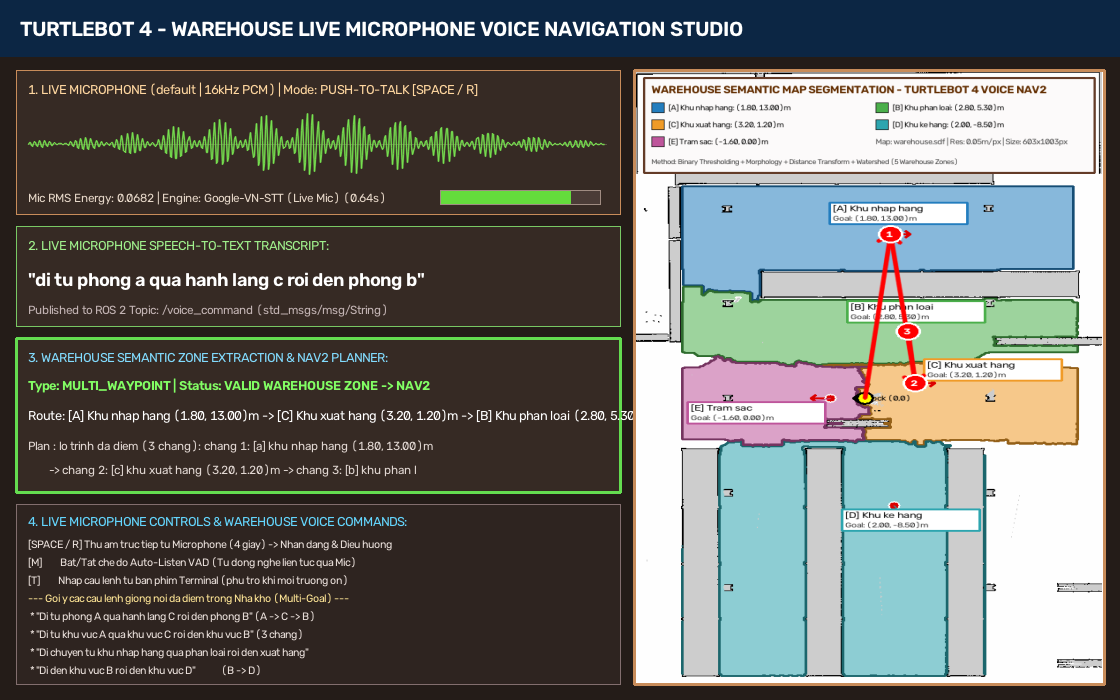
\includegraphics[width=0.62\textwidth]{figures/speech_recognition_demo.png}
  \vspace{-8pt}
  \caption{\footnotesize Giao diện \textit{Warehouse Live Microphone Voice Navigation Studio} khi thu câu lệnh đa điểm trực tiếp từ Microphone: hiển thị sóng âm thời gian thực, phân tích lộ trình đa trạm tuần tự và vẽ đường đi dự kiến.}
  \label{fig:studio}
\end{figure}
\vspace{-8pt}

\begin{table}[H]
  \centering
  \scriptsize
  \caption{\footnotesize Kết quả thực nghiệm nhận dạng câu lệnh giọng nói trực tiếp qua Microphone và điều hướng đa điểm với Nav2.}
  \vspace{-3pt}
  \renewcommand{\arraystretch}{1.06}
  \begin{tabularx}{\textwidth}{c p{4.2cm} c c R}
    \toprule
    \rowcolor{tablehead}
    \textbf{TT} & \textbf{Câu lệnh giọng nói qua Microphone} & \textbf{Loại lệnh} & \textbf{Lộ trình Waypoints} & \textbf{Hành vi thực thi trên hệ thống Nav2} \\
    \midrule
    1 & \textit{``qua A qua B qua C qua D rồi qua E''} & \texttt{MULTI\_WAYPOINT} & $[\text{A} \rightarrow \text{B} \rightarrow \text{C} \rightarrow \text{D} \rightarrow \text{E}]$ & Tuần tự 5 trạm: Nhập hàng $\rightarrow$ Phân loại $\rightarrow$ Xuất hàng $\rightarrow$ Kệ hàng $\rightarrow$ Sạc \\
    2 & \textit{``Đi từ phòng A qua hành lang C rồi đến phòng B''} & \texttt{MULTI\_WAYPOINT} & $[\text{A} \rightarrow \text{C} \rightarrow \text{B}]$ & Điều hướng 3 chặng qua A, C rồi đến B, vẽ lộ trình lên RViz2 \\
    3 & \textit{``Di chuyển từ khu vực B đến khu vực C''} & \texttt{MULTI\_WAYPOINT} & $[\text{B} \rightarrow \text{C}]$ & Đi qua Khu phân loại (B) trước khi tới Khu xuất hàng (C) \\
    4 & \textit{``Đi đến khu nhập hàng''} & \texttt{SINGLE\_GOAL} & $[\text{A}]$ & Điều hướng trực tiếp tới Khu nhập hàng phía Bắc $(1.80, 13.00)\text{ m}$ \\
    5 & \textit{``Quay về trạm sạc''} & \texttt{SINGLE\_GOAL} & $[\text{E}]$ & Trở về Dock sạc tự động tại vị trí trung tâm $(-1.60, 0.00)\text{ m}$ \\
    6 & \textit{``qua A qua B qua C qua Z rồi qua E''} & \texttt{INVALID\_REGION} & $\varnothing$ & Phát hiện vùng \texttt{Z} không tồn tại, từ chối toàn bộ lộ trình, cảnh báo an toàn \\
    \bottomrule
  \end{tabularx}
\end{table}
\vspace{-2pt}

\textbf{Kết luận:} Hệ thống hoàn thiện khả năng nhận dạng giọng nói từ microphone thời gian thực, phân tích chuỗi lệnh phức tạp với $N$ điểm dừng liên hoàn (\textit{``qua A qua B qua C qua D rồi qua E''}), trực quan hóa đường đi dự kiến trên cả RViz2 (\texttt{/voice\_nav/planned\_path}) lẫn cửa sổ bản đồ riêng, đảm bảo robot TurtleBot 4 vận hành an toàn và linh hoạt trong kho vận.

\end{document}
